\chapter{Design}
\subsection{<for mobiles>}
When designing a mobile app with UX focus, the unique challenges of the mobile platform has to be considered. A brief look at three of the most outstanding challenges:
\begin{itemize}
\item Screen size\\
as opposed to a traditional computer screen the general mobile platform has a much more limited amount of screen space. This restriction will force the designers to eliminate as many redundancies as possible so as to not clutter the screen with unnecessary information. \cite{Sardo}
\item User input\\
user input is according to Giorgio Sardo one of  the smartphones weakness. it is mentioned that “Entering text on a mobile phone is hard, and people tend to avoid it if they can”\cite{Sardo}
\item Loading times\\
Mobile devices are generally slower than a PC or Mac, both when it comes to processing power and internet speed, assuming they’re using a mobile network \cite{MobileUsability}
\end{itemize}

Some of the guidelines for optimizing for mobile devices are cutting features, reduce word count and enlarge interface elements to accommodate the “fat finger problem”.\cite{MobileUsability} an example of poor simplification used in the book is IKEA where they simplify the mobile site by only showing a single item when browsing for bedframes.

\begin{figure}[H]
\centering
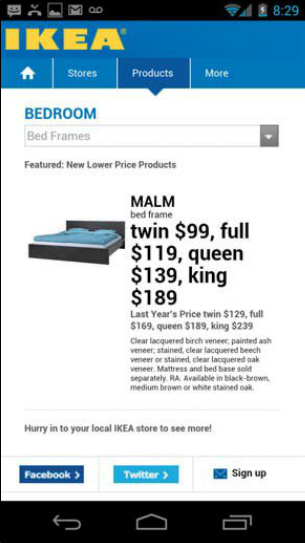
\includegraphics[scale=0.5]{IkeaBadMobile.png}
\caption{the mobile website from IKEA, anno 2013}
\end{figure}

\subsection{Design of 3D testing area}
To test different non-traditional control schemes 3D test area was designed. It consists of twisted path that test participants had to walk through as fast as possible \ref{TestLevels}.
\begin{figure}[H]
\centering
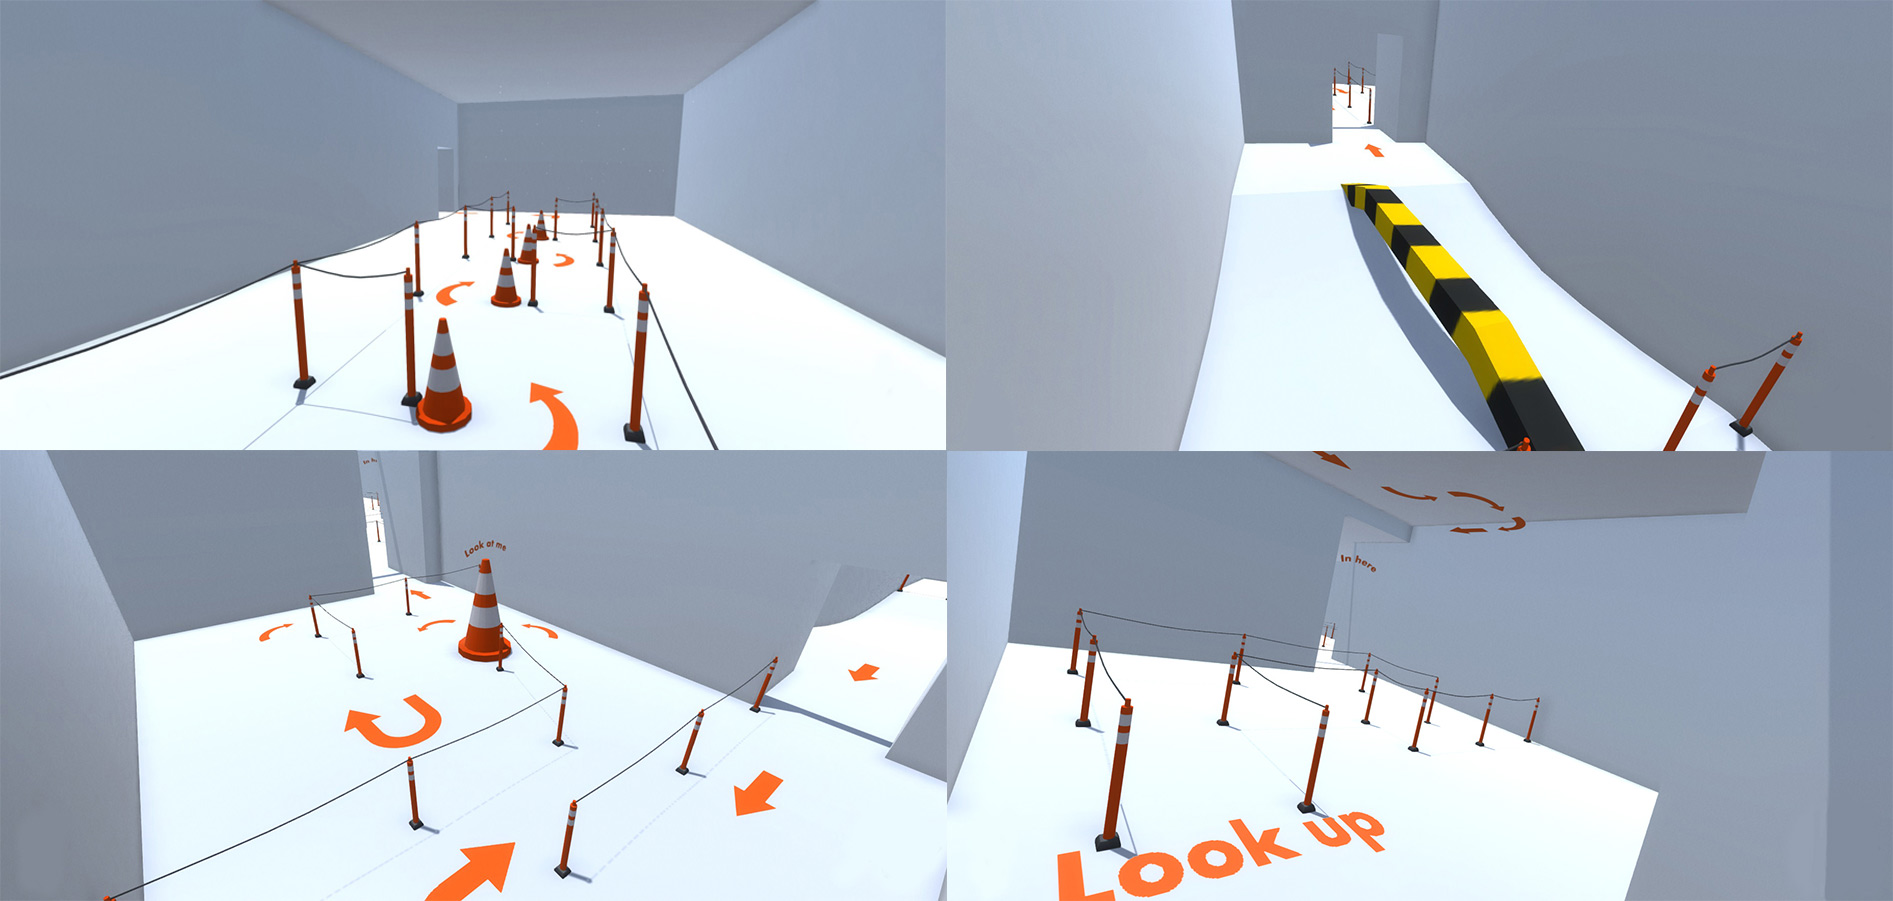
\includegraphics[scale=0.26]{3D_dev_6.jpg}
\caption{Pictures of the testing area}
\label{TestLevels}
\end{figure}
Focus of testing area was only on navigation for different schemes, so effort was placed on path and tasks and not on environment itself. All not important bits of the area were colored white and important as navigational arrows, cones and poles, explanatory text notes colored with sharp contrasting colors as red and orange. The “familiarity” consideration was done - navigational buttons and important bits on the level were kept in similar color, to help user recognize and focus on the purpose.
Analysing SOTA’s applications gave understanding what important aspects of navigation is. Firstly walking fluently around obstacles as furniture, doors, narrow paths. First two levels were developed for this to test. Second consideration was that users need to look around placed furniture which was not considered in most SOTA analyzed applications. Small area with huge cone and text “look at me” was placed and arrows in circular path around it. This represents how user would walk around furniture and inspect it by looking - focusing on one point while walking around \ref{TestLevel3}.
\begin{figure}[H]
\centering
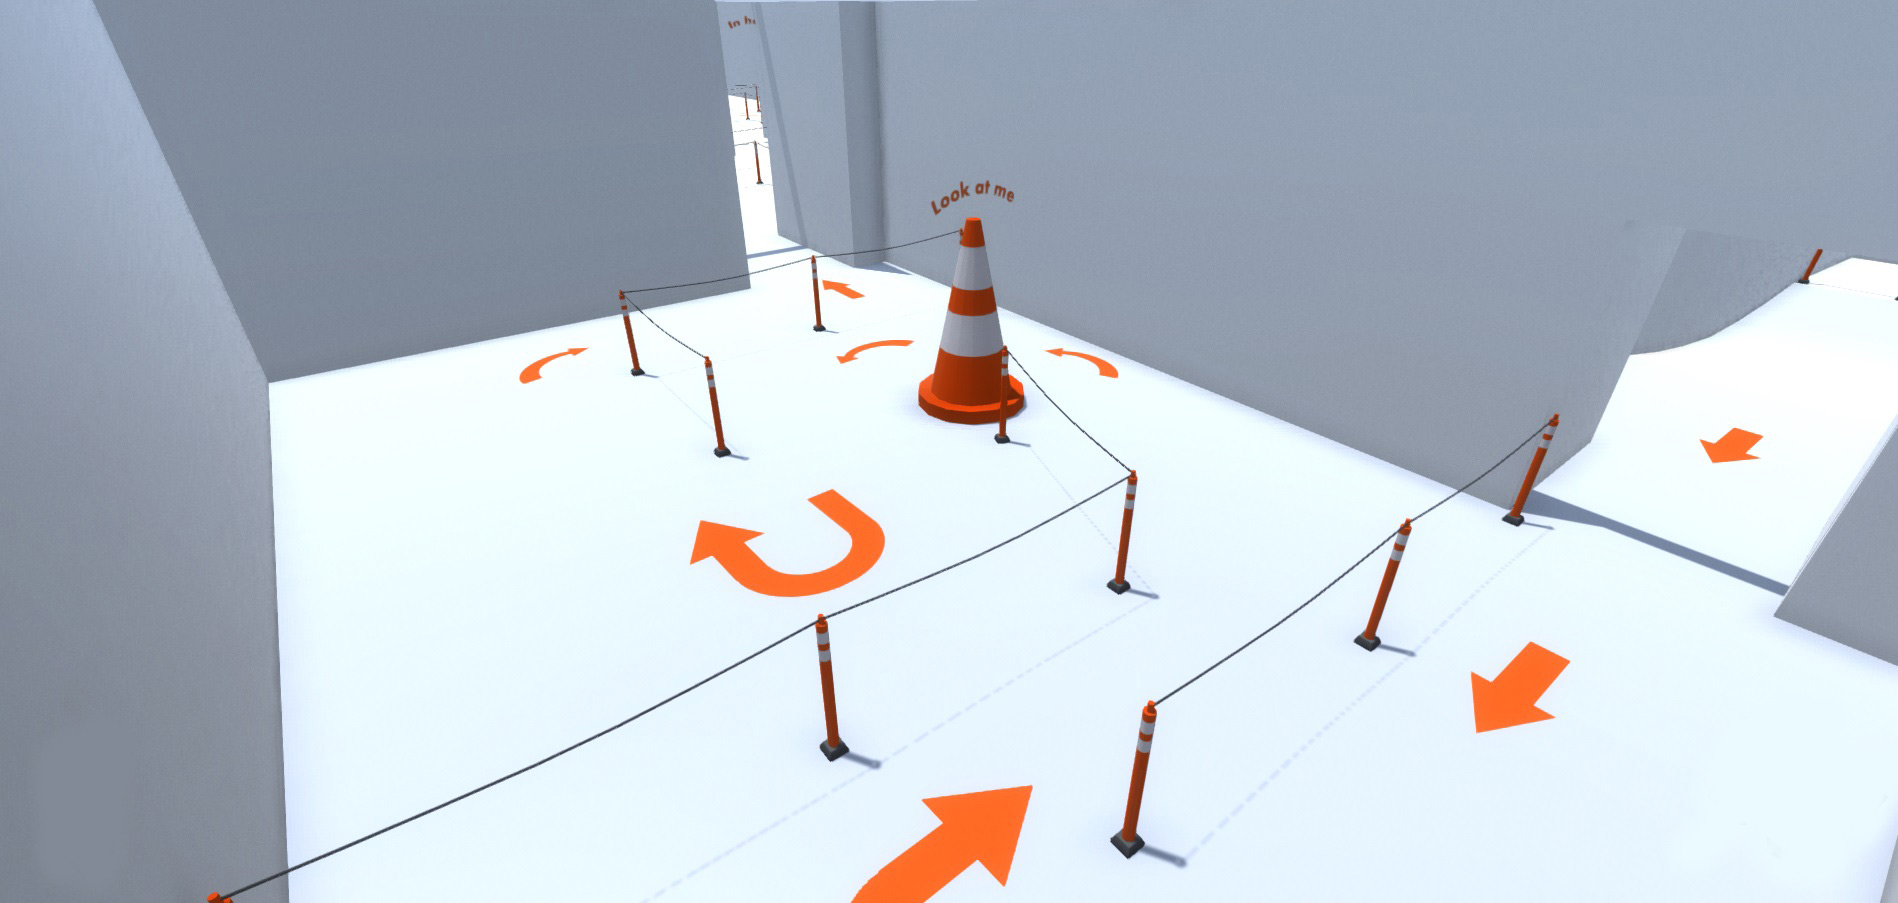
\includegraphics[scale=0.25]{3D_dev_3.jpg}
\caption{Third level of testing area. This level is to test how well user walks around an object.}
\label{TestLevel3}
\end{figure}
Next two levels were developed to test how efficient it is to look up and down while walking in given direction. It helps to test how well user can walk and look down or up at the same time \ref{TestLevel4}.
\begin{figure}[H]
\centering
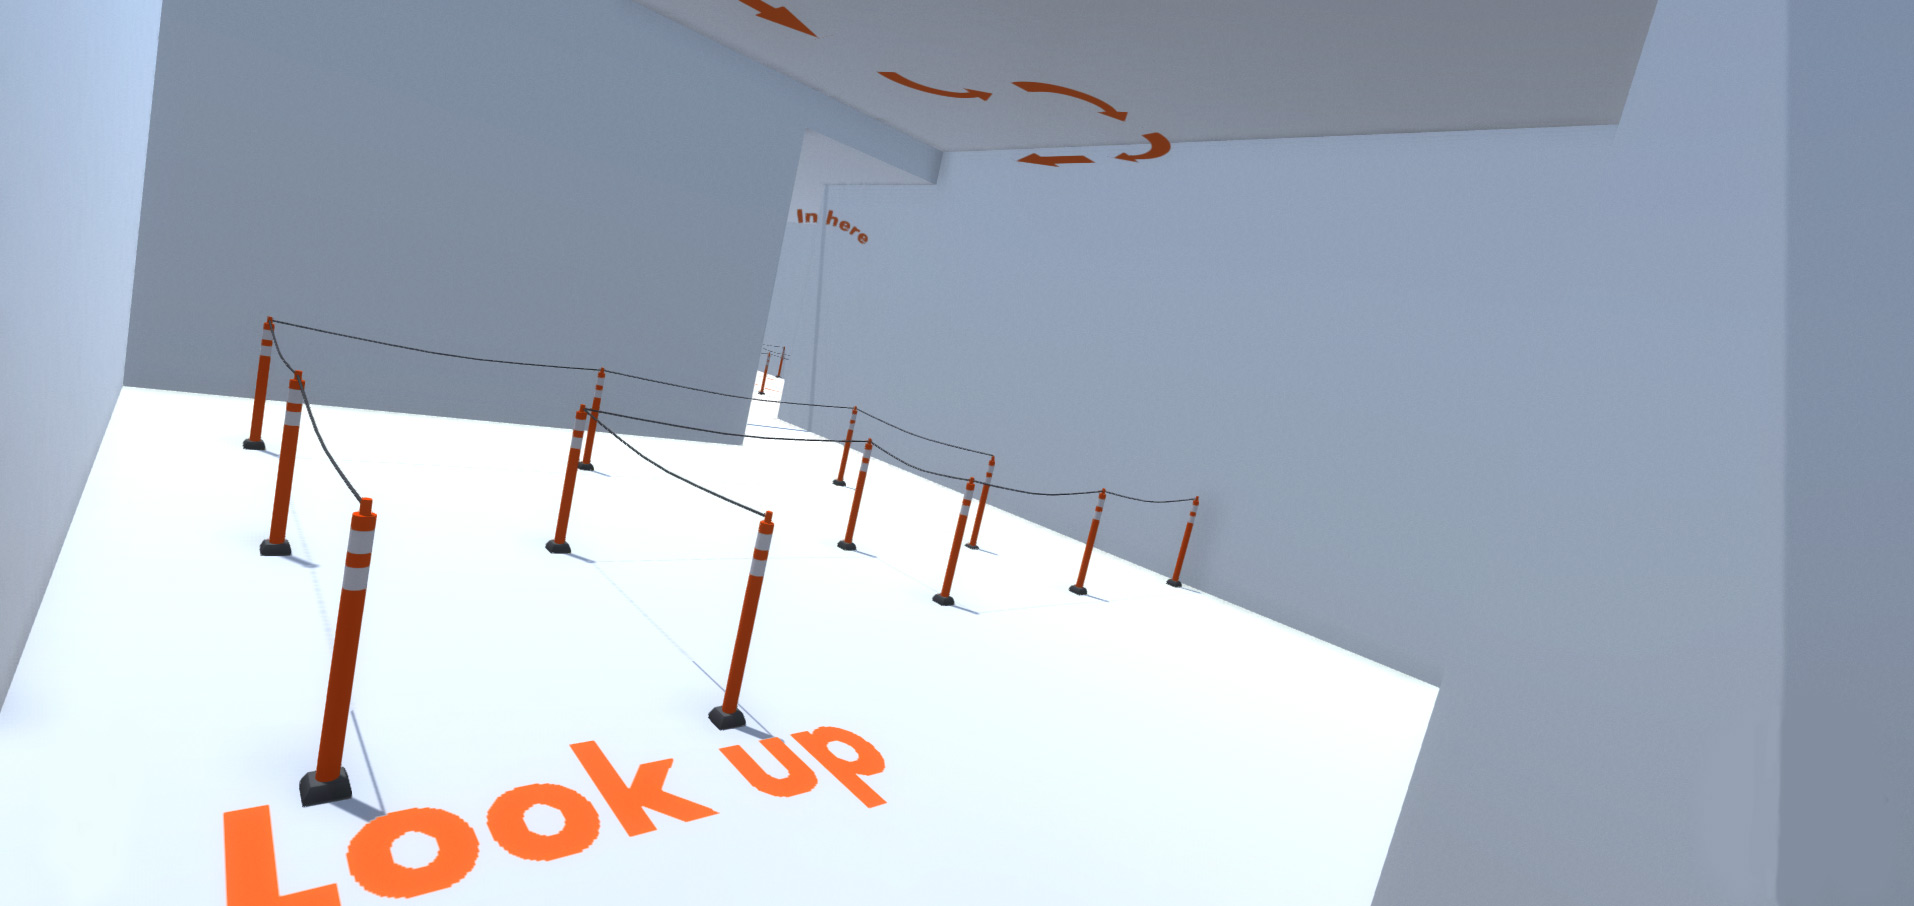
\includegraphics[scale=0.25]{3D_dev_4.jpg}
\caption{Test chamber to test how well user can walk and look up}
\label{TestLevel4}
\end{figure}
The last test area was created to see how user goes straight but looks to one side as the user would walk-by, but focus at some furniture aside \ref{TestLevel5}.
\begin{figure}[H]
\centering
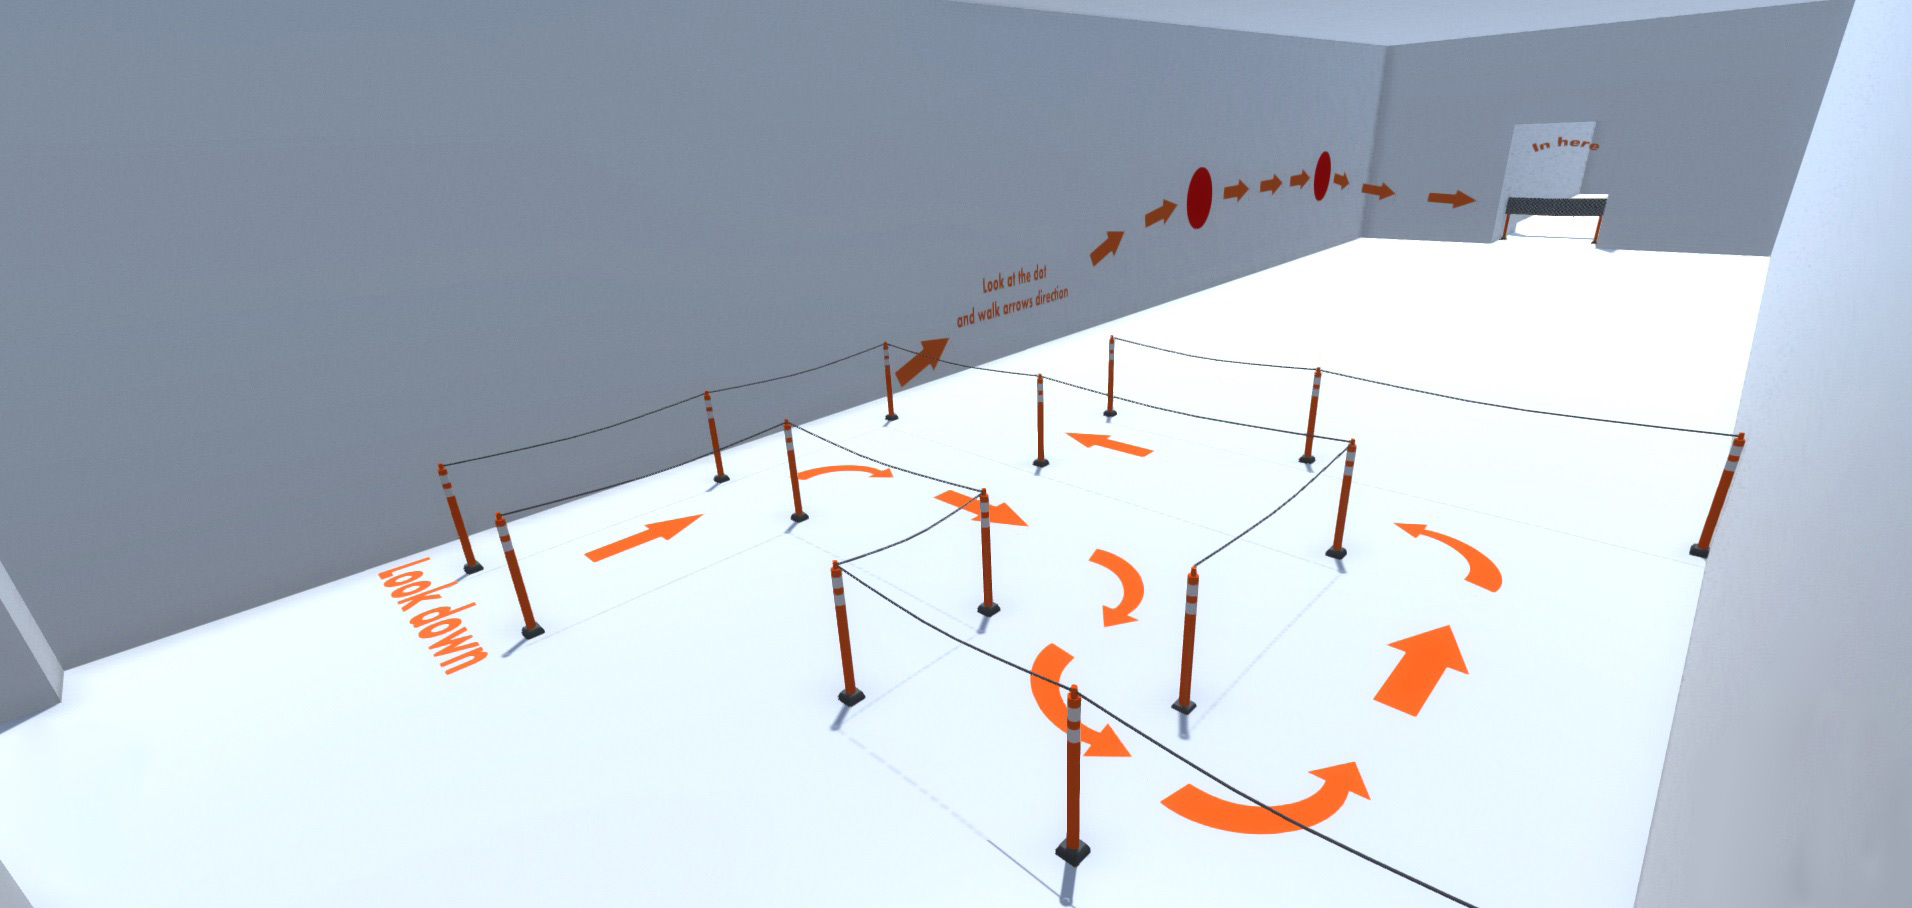
\includegraphics[scale=0.25]{3D_dev_5.jpg}
\caption{Last level of testing area. This level is to test how well user can walk while looking down and sideways}
\label{TestLevel5}
\end{figure}